\documentclass[tikz, border=2pt]{standalone}

\usepackage{amsmath,amssymb}
\usepackage{pgfplots}
\pgfplotsset{compat=1.18}
\usepgfplotslibrary{groupplots}
\usetikzlibrary{arrows.meta}
\usepackage{xcolor}

\definecolor{utnblue}{RGB}{0, 51, 102}
\definecolor{utnred}{RGB}{204, 0, 0}

\begin{document}
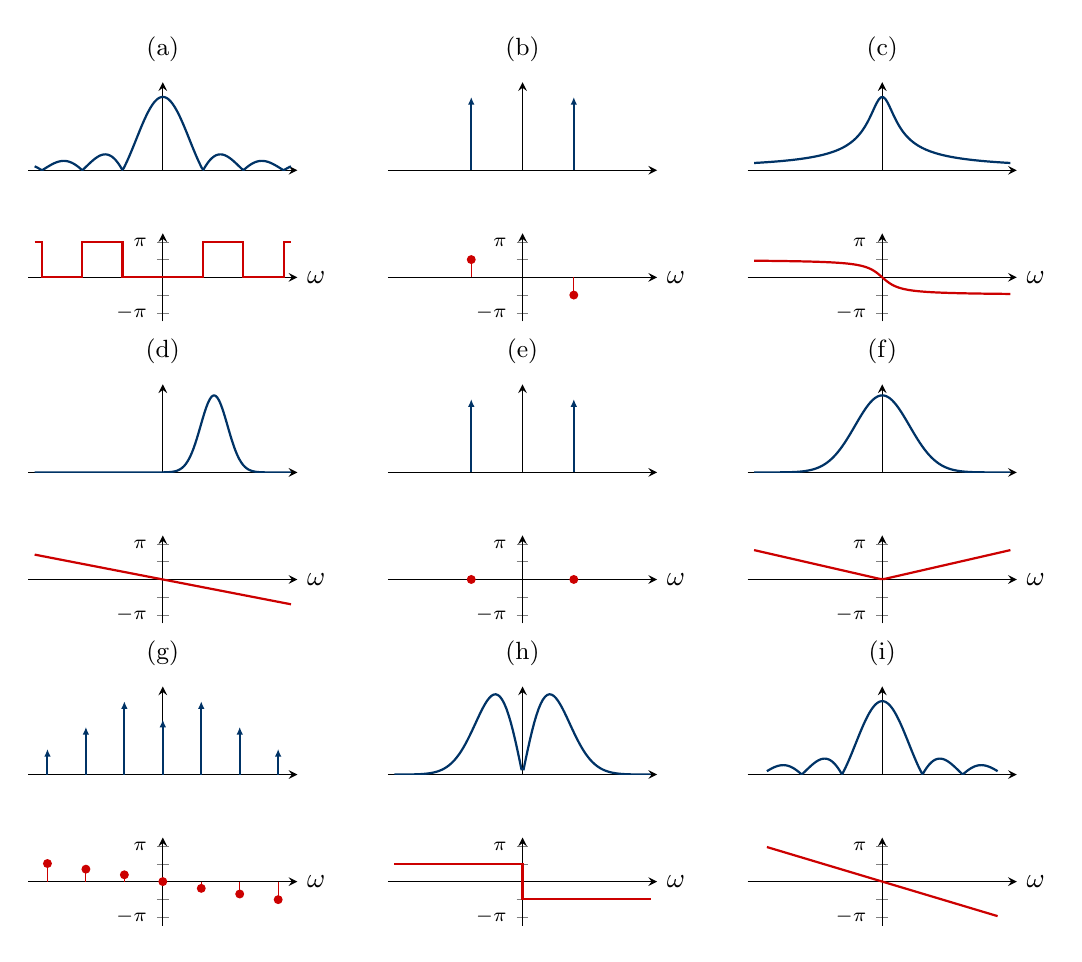
\begin{tikzpicture}[
    impulso/.style={utnblue, line width=0.7pt, -{Latex[length=2.8pt,width=2.4pt]}},
  ]

\pgfplotsset{
  every axis/.append style={
    axis lines=middle,
    width=5.0cm, height=2.7cm,
    enlargelimits=false,
    tick label style={font=\scriptsize},
    title style={font=\small, yshift=-0.5ex},
    label style={font=\scriptsize},
    every axis x label/.style={at={(ticklabel* cs:1)}, anchor=west},
    clip mode=individual,
  },
  modaxis/.style={
    ymin=0, ymax=2.4, ytick=\empty, xtick=\empty,
    xmin=-10.5, xmax=10.5,
  },
  faseaxis/.style={
    ymin=-3.9, ymax=3.9,
    ytick={-3.1416,-1.5708,0,1.5708,3.1416},
    yticklabels={$-\pi$,,$0$,,$\pi$},
    xtick=\empty,
    xmin=-10.5, xmax=10.5,
    xlabel={$\omega$},
  },
}

\begin{groupplot}[
    group style={group size=3 by 6,
                 horizontal sep=1.15cm, vertical sep=0.8cm},
]

% ======================= BANDA 1 : casos (a) (b) (c) =======================
% ---- (a) |X| : pulso (real par) -> sinc, modulo par
\nextgroupplot[modaxis, title={(a)}]
\addplot[utnblue, thick, samples=200, domain=-10:10] {abs(2*sin(deg(x))/x)};

% ---- (b) |X| : seno periodico (real impar) -> dos impulsos iguales
\nextgroupplot[modaxis, title={(b)}]
\draw[impulso] (axis cs:-4,0) -- (axis cs:-4,2.0);
\draw[impulso] (axis cs: 4,0) -- (axis cs: 4,2.0);

% ---- (c) |X| : real ni par ni impar -> exponencial causal
\nextgroupplot[modaxis, title={(c)}]
\addplot[utnblue, thick, samples=120, domain=-10:10] {2/sqrt(1+x*x)};

% ---- (a) fase : 0 / pi (par) -> real par
\nextgroupplot[faseaxis]
\addplot[utnred, thick] coordinates {
  (-10,3.1416) (-9.4248,3.1416) (-9.4248,0) (-6.2832,0)
  (-6.2832,3.1416) (-3.1416,3.1416) (-3.1416,0) (3.1416,0)
  (3.1416,3.1416) (6.2832,3.1416) (6.2832,0) (9.4248,0)
  (9.4248,3.1416) (10,3.1416)
};

% ---- (b) fase : +pi/2 / -pi/2 (impar) -> real impar  [impulsos]
\nextgroupplot[faseaxis]
\draw[utnred, thin] (axis cs:-4,0) -- (axis cs:-4,1.5708);
\draw[utnred, thin] (axis cs: 4,0) -- (axis cs: 4,-1.5708);
\addplot[only marks, mark=*, mark size=1.4pt, utnred]
    coordinates {(-4,1.5708) (4,-1.5708)};

% ---- (c) fase : -arctan(omega) (impar, suave) -> real
\nextgroupplot[faseaxis]
\addplot[utnred, thick, samples=120, domain=-10:10] {-atan(x)*pi/180};

% ======================= BANDA 2 : casos (d) (e) (f) =======================
% ---- (d) |X| : modulo NO par -> no real
\nextgroupplot[modaxis, title={(d)}]
\addplot[utnblue, thick, samples=140, domain=-10:10] {2.1*exp(-(x-4)*(x-4)/2.2)};

% ---- (e) |X| : coseno periodico (real par) -> dos impulsos iguales
\nextgroupplot[modaxis, title={(e)}]
\draw[impulso] (axis cs:-4,0) -- (axis cs:-4,2.0);
\draw[impulso] (axis cs: 4,0) -- (axis cs: 4,2.0);

% ---- (f) |X| : modulo par
\nextgroupplot[modaxis, title={(f)}]
\addplot[utnblue, thick, samples=120, domain=-10:10] {2.1*exp(-x*x/9)};

% ---- (d) fase : impar, pero el modulo no es par -> no real
\nextgroupplot[faseaxis]
\addplot[utnred, thick, domain=-10:10] {-0.22*x};

% ---- (e) fase : 0 en los impulsos (par) -> real par
\nextgroupplot[faseaxis]
\addplot[only marks, mark=*, mark size=1.4pt, utnred]
    coordinates {(-4,0) (4,0)};

% ---- (f) fase : PAR (no impar) -> no real
\nextgroupplot[faseaxis]
\addplot[utnred, thick, samples=80, domain=-10:10] {0.26*abs(x)};

% ======================= BANDA 3 : casos (g) (h) (i) =======================
% ---- (g) |X| : periodica con varios armonicos (real) -> impulsos pares
\nextgroupplot[modaxis, title={(g)}]
\draw[impulso] (axis cs: 0,0) -- (axis cs: 0,1.5);
\draw[impulso] (axis cs:-3,0) -- (axis cs:-3,2.0);
\draw[impulso] (axis cs: 3,0) -- (axis cs: 3,2.0);
\draw[impulso] (axis cs:-6,0) -- (axis cs:-6,1.3);
\draw[impulso] (axis cs: 6,0) -- (axis cs: 6,1.3);
\draw[impulso] (axis cs:-9,0) -- (axis cs:-9,0.7);
\draw[impulso] (axis cs: 9,0) -- (axis cs: 9,0.7);

% ---- (h) |X| : real impar -> modulo par con cero en el origen
\nextgroupplot[modaxis, title={(h)}]
\addplot[utnblue, thick, samples=120, domain=-10:10] {1.7*abs(x)*exp(-x*x/9)};

% ---- (i) |X| : sinc (modulo par) -> pulso desplazado
\nextgroupplot[modaxis, title={(i)}]
\addplot[utnblue, thick, samples=200, domain=-9:9] {abs(2*sin(deg(x))/x)};

% ---- (g) fase : impar (varios armonicos) -> real
\nextgroupplot[faseaxis]
\draw[utnred, thin] (axis cs:-3,0) -- (axis cs:-3,0.6);
\draw[utnred, thin] (axis cs: 3,0) -- (axis cs: 3,-0.6);
\draw[utnred, thin] (axis cs:-6,0) -- (axis cs:-6,1.1);
\draw[utnred, thin] (axis cs: 6,0) -- (axis cs: 6,-1.1);
\draw[utnred, thin] (axis cs:-9,0) -- (axis cs:-9,1.6);
\draw[utnred, thin] (axis cs: 9,0) -- (axis cs: 9,-1.6);
\addplot[only marks, mark=*, mark size=1.4pt, utnred]
    coordinates {(0,0) (-3,0.6) (3,-0.6) (-6,1.1) (6,-1.1) (-9,1.6) (9,-1.6)};

% ---- (h) fase : +pi/2 / -pi/2 (impar) -> real impar
\nextgroupplot[faseaxis]
\addplot[utnred, thick] coordinates {
  (-10,1.5708) (0,1.5708) (0,-1.5708) (10,-1.5708)
};

% ---- (i) fase : rampa lineal (impar) -> real, retardo puro
\nextgroupplot[faseaxis]
\addplot[utnred, thick, domain=-9:9] {-0.34*x};

\end{groupplot}

\end{tikzpicture}
\end{document}
